% Made up for the tikra benchmark.
\usetikzlibrary{shapes.callouts}
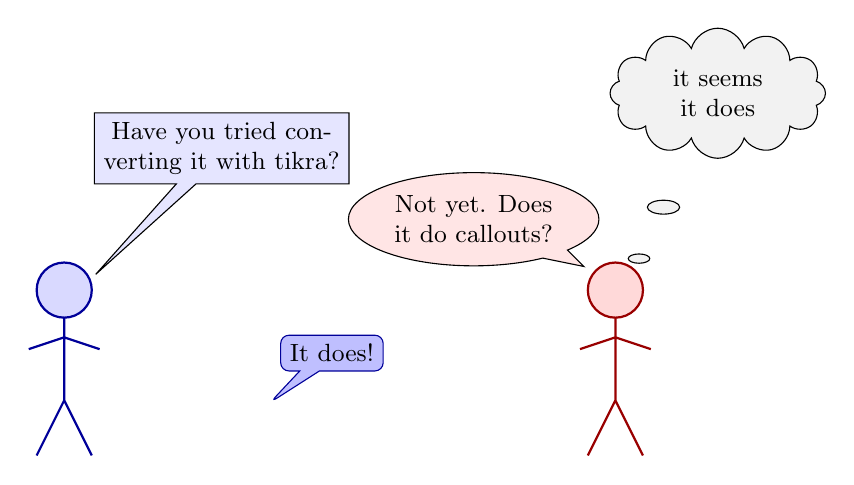
\begin{tikzpicture}[font=\small]
  % two stick figures talking
  \foreach \x/\c in {0/blue, 7/red} {
    \draw[\c!60!black, thick, fill=\c!15] (\x,0.4) circle (0.35);
    \draw[\c!60!black, thick] (\x,0.05) -- (\x,-1) (\x-0.45,-0.35) -- (\x,-0.2) -- (\x+0.45,-0.35)
      (\x-0.35,-1.7) -- (\x,-1) -- (\x+0.35,-1.7);
  }
  \node[rectangle callout, draw, fill=blue!10, callout absolute pointer={(0.4,0.6)}, text width=3cm, align=center]
    at (2,2.2) {Have you tried converting it with tikra?};
  \node[ellipse callout, draw, fill=red!10, callout absolute pointer={(6.6,0.7)}, align=center]
    at (5.2,1.3) {Not yet. Does\\it do callouts?};
  \node[cloud callout, draw, fill=gray!10, cloud puffs=12, aspect=2.2, callout absolute pointer={(7.3,0.8)}, align=center]
    at (8.3,2.9) {it seems\\it does};
  \node[rectangle callout, draw=blue!60!black, fill=blue!25, rounded corners=3pt,
        callout relative pointer={(-0.5,-0.4)}] at (3.4,-0.4) {It does!};
\end{tikzpicture}
